% !TeX root=tukedip.tex
% !TeX encoding = UTF-8
% !TeX spellcheck = sk_SK
\section{Analýza súčasného stavu}
Pred výberom metódy optického polohovania a navigácie sme museli preskúmať rôzne možnosti. Pozreli sme sa na metódy, ktoré by mohli byť vhodné na navigáciu dronov. Skúmala sa ich použiteľnosť pre mikrodrony.

\subsection{Optický princíp senzorov}
Snímače s optickým princípom sa bežne používajú v mobilnej robotike na navigáciu, lokalizáciu a mapovanie. Tieto senzory zachytávajú informácie z prostredia analýzou svetla a jeho interakcie s povrchmi, čím poskytujú bohaté údaje na presné určovanie polohy robota a plánovanie trajektórie. V tejto časti sa budeme zaoberať rôznymi typmi optických principiálnych snímačov a ich aplikáciami v mobilnej robotike \citep{Li2022}.

Jedným z najčastejšie používaných optických snímačov je kamera, ktorá zachytáva obrázky a videá prostredia. Kamery poskytujú bohaté vizuálne informácie vrátane farby, textúry a tvaru, ktoré možno využiť na detekciu, sledovanie a rozpoznávanie objektov. V našej práci využívame kamery namontované na bezpilotných lietadlách Tello na zisťovanie polohy značiek Aruco a odhadovanie ich súradníc v 3D priestore \citep{Li2022}. 

Ďalším dôležitým optickým senzorom je senzor LIDAR (Light Detection and Ranging), ktorý vysiela laserové lúče a meria ich odraz na vytvorenie 3D mapy prostredia. Senzory LIDAR sa bežne používajú v autonómnych vozidlách na vyhýbanie sa prekážkam a mapovanie. Sú však drahé a vyžadujú vysoký výpočtový výkon, čo ich robí menej vhodnými pre malú mobilnú robotiku \citep{Takahashi2014}.
 
Okrem kamier a LIDAR-u patria medzi ďalšie typy snímačov na optickom princípe infračervené snímače, ultrazvukové snímače a snímače času letu. Infračervené senzory merajú odraz infračerveného svetla na detekciu objektov a meranie ich vzdialenosti, zatiaľ čo ultrazvukové senzory vysielajú vysokofrekvenčné zvukové vlny a merajú ich ozvenu na odhad vzdialenosti. Snímače času letu využívajú svetlo na meranie času, za ktorý sa signál odrazí späť, čím poskytujú presné merania vzdialenosti.

Senzory na optickom princípe celkovo zohrávajú kľúčovú úlohu v mobilnej robotike a poskytujú bohaté informácie na navigáciu a lokalizáciu robota. Pochopením rôznych typov senzorov a ich aplikácií môžeme navrhnúť a implementovať efektívne robotické systémy, ktoré môžu fungovať v rôznych prostrediach a scenároch.

\subsection{Vyhýbanie sa prekážkam a orientácia na základe obrazu z kamery}
Jedným z najdôležitejších úloh mobilných robotov je schopnosť vyhnúť sa prekážkam a správne sa orientovať v prostredí. K dispozícii sú rôzne senzory, ktoré umožňujú robotom rozpoznať a vyhnúť sa prekážkam. Okrem senzorov ako LIDAR, ultrazvukových a infračervených senzorov sa dá využiť aj obraz z kamery.

Kamera poskytuje bohaté vizuálne informácie o prostredí a umožňuje robotom získavať informácie o prekážkach a teréne. Existujú rôzne spôsoby, ako využiť obraz z kamery pre navigáciu a vyhýbanie sa prekážkam.

\subsubsection{Prístup s vylepšenou neurónovou sieťou}
Jednou zo skúmaných metód na vyhýbanie sa prekážkam a orientáciu pomocou kamery bolo strojové učenie pomocou neurónových sietí. Nakoniec však bola zavrhnutá kvôli časovo a hardvérovo náročným procesom učenia. Táto metóda zahŕňa použitie naučenej neurónovej siete na priradenie približných hodnôt hĺbky každému pixelu na základe polohy objektov z jedného obrazu. Vzory sa dajú naučiť z dvojice LIDAR a digitálnych kamier umiestnených vedľa seba. Zadaním dostatočného počtu týchto naučených dvojíc môže neurónová sieť vytvoriť vzťah medzi pixelmi na obrázkoch a hodnotami hĺbky získanými z LIDAR-u alebo stereokamery.

Sieť sa môže učiť pomocou učenia založeného na LIDAR-e s dohľadom a učenia založeného na stereopároch bez dohľadu na základe pravdepodobnostného princípu. Učenie pod dohľadom je však často príliš prísne a učenie bez dohľadu poskytuje nepresné výsledky. Preto sa odporúča používať poloprevádzkové učenie alebo porovnávať výsledky získané pomocou siete s kalibrovaným systémom detekcie hĺbky počas prevádzky \citep{xie2016edge}.

Táto metóda získava hodnoty hĺbky z okolia a umiestnenia objektov (množiny pixelov) a vytvára mapu hĺbky podobnú tej, ktorá je znázornená na obrázku 2-1. Jej presnosť je zatiaľ experimentálna a takýto systém je stále vystavený mnohým chybám. Napriek tomu bol použitý v aplikáciách na riadenie dronov. Hĺbkové mapy na obrázku 1 ilustrujú rozdiel medzi rôznymi metódami a presnosť tejto metódy \citep{ikeoka2018depth, xie2016edge}.

\begin{figure}[ht!]
    \centering
    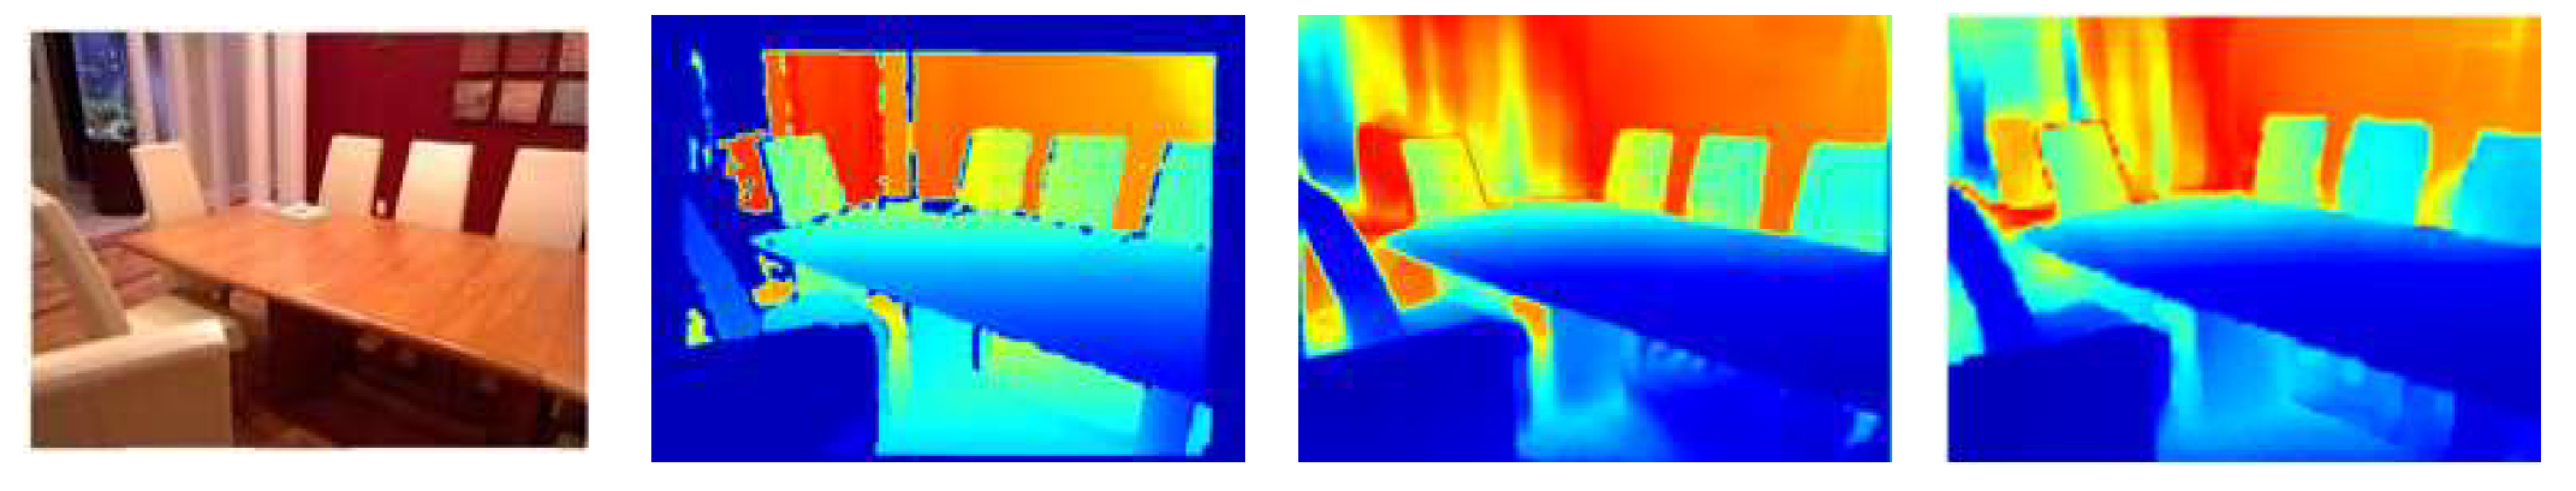
\includegraphics[width=.85\textwidth,angle=0]{figure 2-1.pdf}
    \caption{Načítaný obraz (vľavo), skutočná mapa hĺbky na základe senzorov (vľavo uprostred) a napokon mapa hĺbky vytvorená pomocou Gaussovho modelu (vpravo uprostred) a Laplaceovho modelu (vpravo)}
    \captionsetup{font=footnotesize, justification=centering, skip=5pt}
    \caption*{(Zdroj: Khan, F., https://doi.org/10.3390/s20082272)}
    \label{o:2-1}
\end{figure}
% Khan, F.; Salahuddin, S.; Javidnia, H. Deep Learning-Based Monocular Depth Estimation Methods—A State-of-the-Art Review. Sensors 2020, 20, 2272. https://doi.org/10.3390/s20082272

Neurónová sieť berie do úvahy niekoľko faktorov(Obrázok. 2-2):
\begin{itemize}
    \item \textbf{oklúzia;}
    \item \textbf{relatívna veľkosť;}
    \item \textbf{vrhaný tieň;}
    \item \textbf{tieňovani;}
    \item \textbf{vzdialenosť od horizontu;}
    \item \textbf{gradient textúry;}
    \item \textbf{lineárna perspektíva.}
\end{itemize}
Učenie siete je časovo a zdrojovo náročné. Po natrénovaní je výzvou zabezpečiť, aby sieť fungovala v reálnom čase na riadenie dronov bez toho, aby sa stratilo príliš veľa údajov v dôsledku zrýchlenia kalibrácie, čo môže viesť ku kolíziám. Počas pomalého letu sa sieť stále dokáže vyhýbať prekážkam, ale považuje ich len za súbor bodov s relatívnou polohou, nie za presné obrysy \citep{aabed2012depth}.

\begin{figure}[ht!]
    \centering
    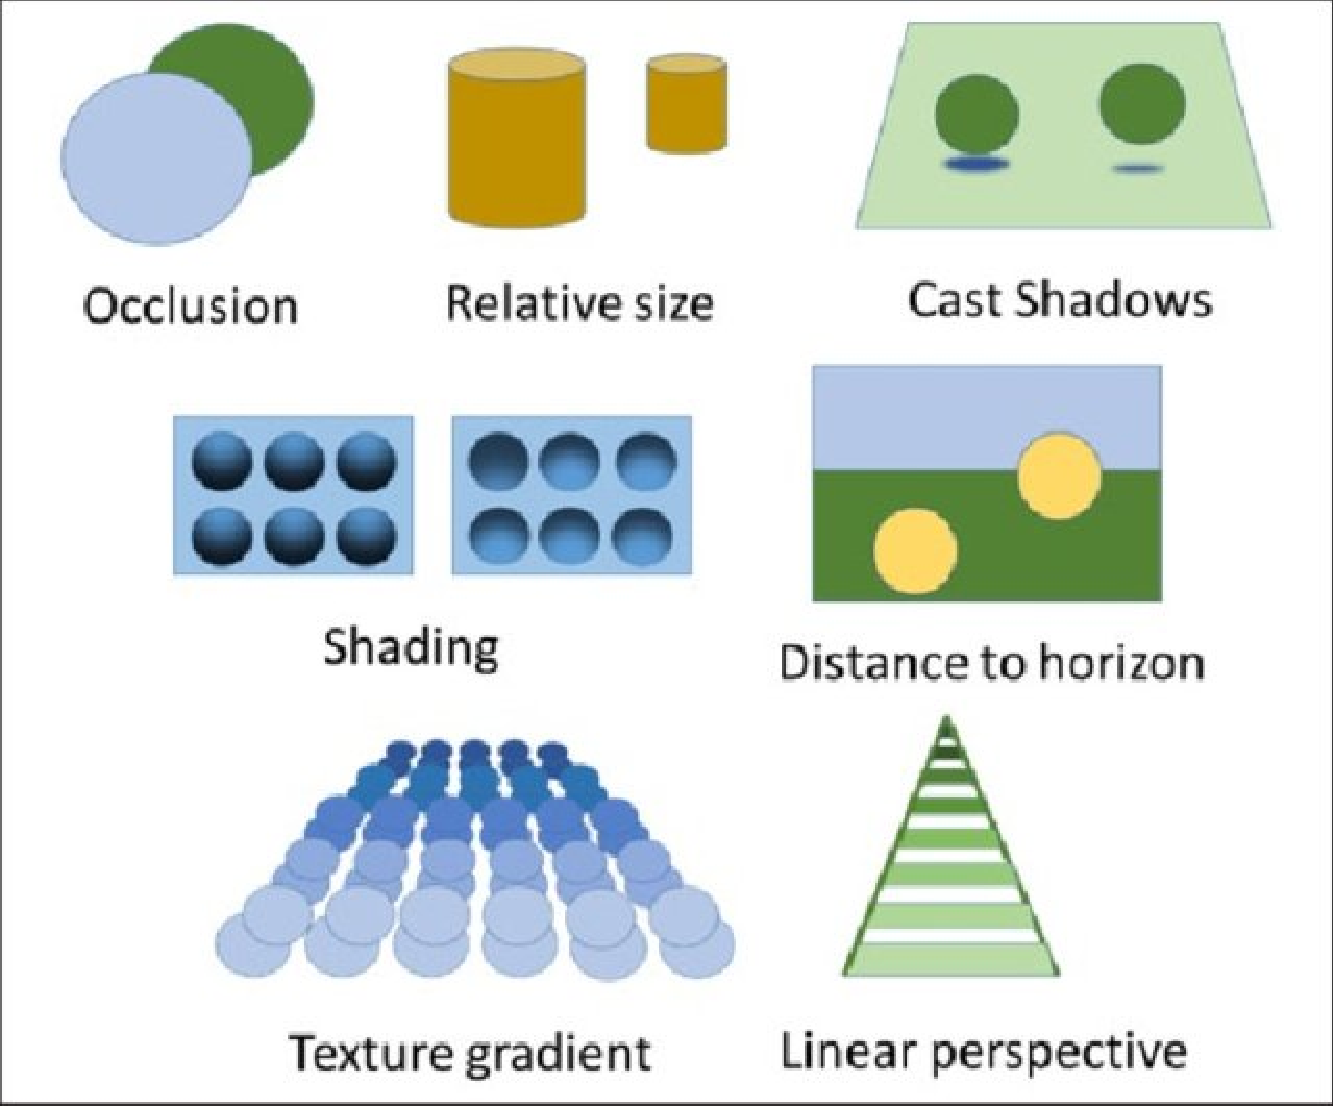
\includegraphics[width=.55\textwidth,angle=0]{figure 2-2.pdf}
    \caption{Faktory zohľadňované pri monokulárnom vnímaní hĺbky}
    \captionsetup{font=footnotesize, justification=centering, skip=5pt}
    \caption*{(Zdroj: Bogdanova (2016). Depth Perception of Surgeons in Minimally Invasive Surgery. Surgical Innovation. 23. 10.1177/1553350616639141.)}
    \label{o:2-2}
\end{figure}
% Bogdanova, Rositsa & Boulanger, Pierre & Zheng, Bin. (2016). Depth Perception of Surgeons in Minimally Invasive Surgery. Surgical Innovation. 23. 10.1177/1553350616639141. 

\subsubsection{Princíp stereosnímania}
Princíp stereosnímania je široko používaná metóda vnímania hĺbky v počítačovom videní, robotike a príbuzných oblastiach. Zahŕňa použitie dvoch alebo viacerých kamier na snímanie obrazov tej istej scény z rôznych uhlov pohľadu a následné použitie rozdielov v obrazoch na výpočet vzdialeností objektov na scéne. Tento princíp sa uplatňuje pri rôznych úlohách v robotike vrátane rozpoznávania objektov, navigácie a vyhýbania sa prekážkam \citep{brzozowski2018stereo}.

V kontexte bezpilotných lietadiel môže byť princíp stereočočočky užitočným nástrojom na navigáciu a vyhýbanie sa prekážkam. Výhodou použitia stereolitografie je, že je k dispozícii mnoho voľne použiteľných riešení, vrátane knižnice OpenCV. Používa sa aj na ovládanie dronov, ale jeho spoľahlivosť pri vysokých rýchlostiach je veľmi nízka. Na vytvorenie hĺbkovej mapy je potrebná dokonalá kalibrácia a pevná fixácia kamery, inak systém poskytne chybné údaje. Naš dron DJI Tello má však napríklad len jednu kameru. V takomto prípade možno obraz z kamery rozdeliť na dve virtuálne kamery, ktoré sa potom môžu použiť na simuláciu stereovidenia, ako je znázornené na obrázku 2-3. Tento prístup má však svoje obmedzenia a výzvy \citep{brzozowski2018stereo}.

\begin{figure}[ht!]
    \centering
    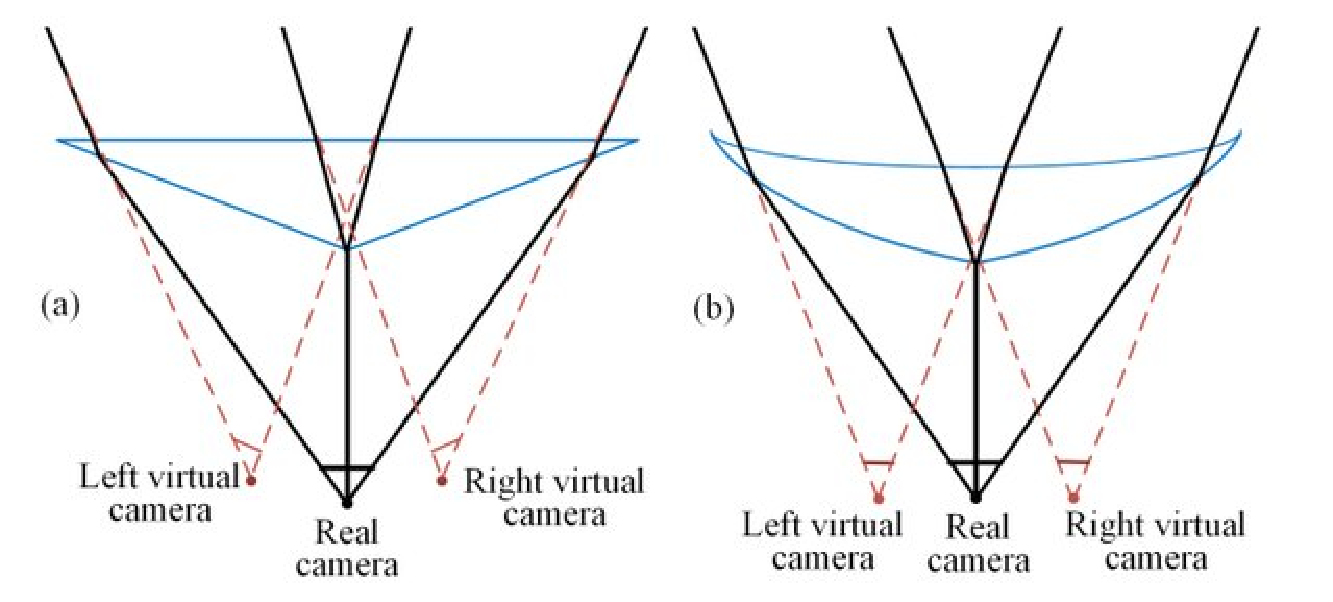
\includegraphics[width=.85\textwidth,angle=0]{figure 2-3.pdf}
    \caption{Model virtuálnej kamery. (a) Model virtuálnej kamery systému stereovízie založeného na plochej prizme. (b) Modifikovaný model dierkovej virtuálnej kamery systému stereovízie založeného na voľnej prizme.}
    \captionsetup{font=footnotesize, justification=centering, skip=5pt}
    \caption*{(Zdroj: Cui. (2019). Design of a Single-Lens Freeform-Prism-Based Distortion-Free Stereovision System. IEEE Photonics Journal. PP. 1-1. 10.1109/JPHOT.2019.2924458)}
    \label{o:2-3}
\end{figure}
%Cui, Xiaoyu & Wang, Liqian & Ren, Yuetian & Chen, Shuo & Zhao, Yue & Lim, Kah-Bin & Gong, Tianxing. (2019). Design of a Single-Lens Freeform-Prism-Based Distortion-Free Stereovision System. IEEE Photonics Journal. PP. 1-1. 10.1109/JPHOT.2019.2924458. 

Jednou z hlavných výziev je, že rozlíšenie virtuálnych kamier je nižšie ako rozlíšenie skutočnej kamery. Toto zníženie rozlíšenia môže ovplyvniť presnosť vnímania hĺbky, najmä v prípade vzdialených objektov. Ďalšou výzvou je, že základná vzdialenosť medzi dvoma virtuálnymi kamerami je pevná a nedá sa upraviť, čo môže obmedziť rozsah vzdialeností, ktoré možno presne odhadnúť \citep{cui2019design}.

Okrem toho výkonnosť princípu stereosnímania môžu ovplyvniť rôzne faktory, ako sú svetelné podmienky, kalibrácia kamery a oklúzie. Tieto faktory môžu mať za následok chyby vo vnímaní hĺbky, čo môže viesť ku kolíziám alebo nepresnej navigácii \citep{cui2019design}.

Vzhľadom na tieto problémy je pochopiteľné, prečo princíp stereosnímania nemusí byť vždy najlepším riešením pre navigáciu dronov. Namiesto toho môžu byť na tieto úlohy vhodnejšie iné techniky.

Na záver možno konštatovať, že hoci je princíp stereosnímania výkonnou metódou na vnímanie hĺbky a úspešne sa uplatňuje v rôznych oblastiach, jeho použitie v kontexte dronov, ako je Tello, je obmedzené z dôvodu použitia iba jednej kamery. V dôsledku toho môže byť potrebné použiť iné techniky snímania v spojení s týmto princípom, aby sa dosiahla presná a spoľahlivá navigácia dronov.

\subsubsection{Prístup na základe pohyblivého obrazu kamery}
Ďalším populárnym prístupom k dosiahnutiu vnímania hĺbky v bezpilotných lietadlách je použitie metód založených na snímaní pohyblivou kamerou. Táto metóda zahŕňa snímanie sekvencie obrazov pomocou jednej kamery namontovanej na dron a následné použitie algoritmov na odhad informácií o hĺbke na základe pohybu kamery.

\begin{figure}[ht!]
    \centering
    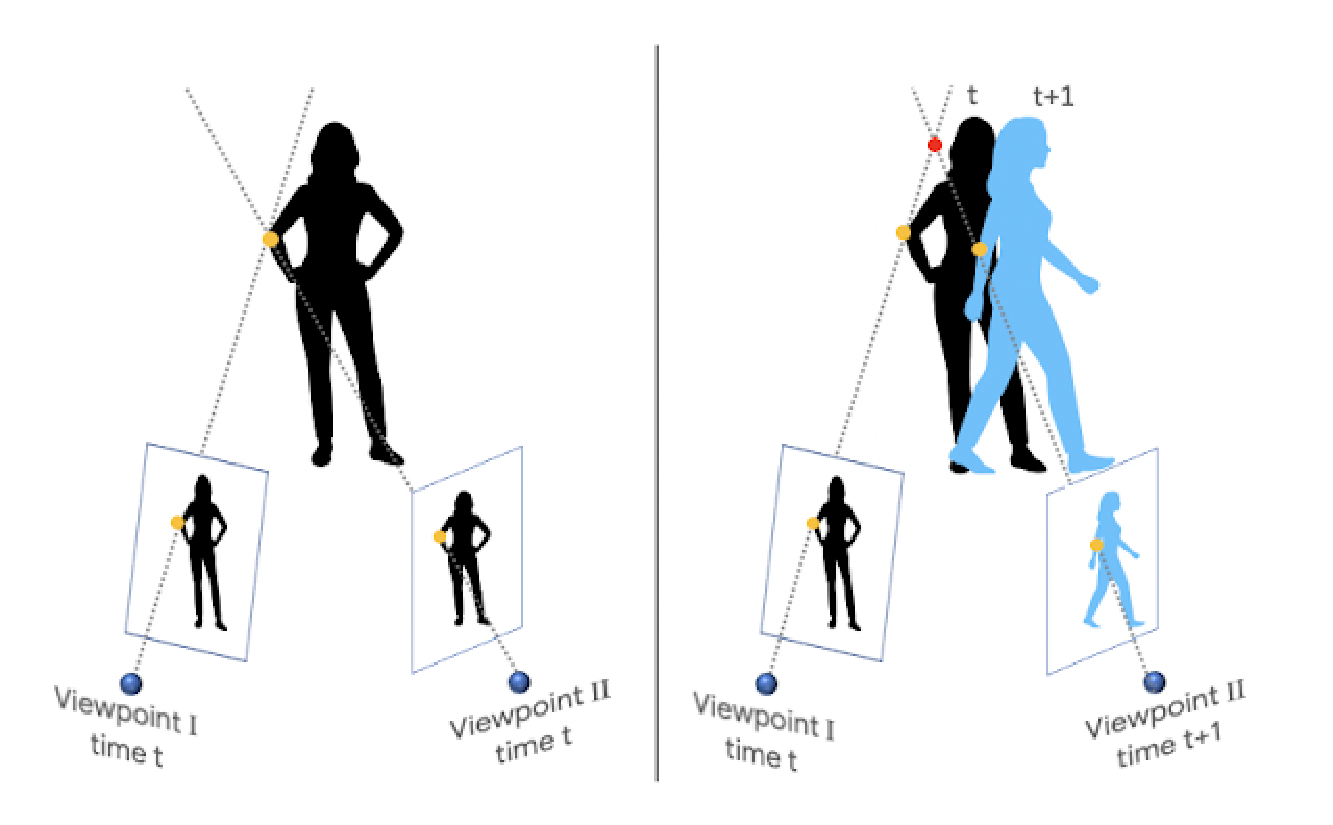
\includegraphics[width=.90\textwidth,angle=0]{figure 2-4.pdf}
    \caption{Vľavo: Tradičné stereofónne nastavenie predpokladá, že aspoň dva uhly pohľadu zachytávajú scénu v rovnakom čase. Vpravo: Uvažujeme o nastavení, pri ktorom sa kamera aj objekt pohybujú.}
    \captionsetup{font=footnotesize, justification=centering, skip=5pt}
    \caption*{(Zdroj: https://ai.googleblog.com/2019/05/moving-camera-moving-people-deep.html)}
    \label{o:2-4}
\end{figure}
%https://ai.googleblog.com/2019/05/moving-camera-moving-people-deep.html

Ide o riešenie, o použití ktorého v našej práci sa uvažovalo dlho. Myšlienka spočíva v tom, že ak nemáte dve kamery, môžete dronom pohybovať a fotografovať objekt z viacerých uhlov, ako je znázornené na obrázku 2-4. Na rozdiel od stereolitografie zhotovujeme desiatky snímok namiesto dvoch a porovnávame pixely medzi sebou a s polohou kamery v čase zhotovenia snímky. Takto môžeme získať hĺbkový obraz na základe viacerých uhlov pohľadu a pozícií kamery. Týmto spôsobom môžeme získať hĺbkový obraz na základe viacerých uhlov pohľadu a pozícií kamery. 
Prekvapujúce bolo, že na základe štúdie Alvareza \citep{alvarez2016collision} chyby polohovania dronu počas vznášania poskytujú dostatočný posun na vytvorenie mapy hĺbky a na získanie potrebných údajov stačí 30 snímok. 

V porovnaní s predchádzajúcimi uvedenými metódami má prístup založený na snímaní pohyblivou kamerou tú výhodu, že nevyžaduje žiadne ďalšie snímače alebo zariadenia. Okrem toho umožňuje väčšiu flexibilitu, pokiaľ ide o umiestnenie a pohyb dronu.

Tento prístup však nie je bez obmedzení. Presnosť informácií o hĺbke získaných touto metódou do veľkej miery závisí od kvality použitých algoritmov na odhad pohybu. Okrem toho je táto metóda náchylná na chyby spôsobené faktormi, ako je rozmazanie pohybu kamery, zlé svetelné podmienky a oklúzia. V tomto
prípade bola táto myšlienka zavrhnutá aj kvôli šumu z akcelerometrov a chybám,
ktoré môžu vzniknúť.

Napriek týmto obmedzeniam sa metóda založená na snímaní pohyblivej kamery úspešne používa v rôznych aplikáciách dronov, ako je vyhýbanie sa prekážkam a mapovanie. V porovnaní s ostatnými už uvedenými metódami môže byť tento prístup pre svoju jednoduchosť a flexibilitu vhodnejší pre určité prípady použitia.

\subsubsection{Určovanie polohy pomocou značiek}
Určovanie polohy pomocou značiek je populárna metóda na presný odhad polohy (pozície a orientácie) kamery vzhľadom na prostredie. Táto metóda zahŕňa umiestnenie značiek so známou geometriou v prostredí a ich detekciu v obrazoch kamery. Značky Aruco, ktoré sú založené na štvorcových čiernobielych vzoroch s jedinečným kódom, sú obľúbenou voľbou pre túto metódu vďaka ich vysokej presnosti a odolnosti voči rôznym svetelným podmienkam \citep{Marut2019}.

Proces používania značiek Aruco na určovanie polohy zahŕňa detekciu značiek v obraze kamery dronu, použitie známej veľkosti a polohy značiek na výpočet polohy a orientácie dronu vzhľadom na značky a následné použitie týchto informácií na navigáciu dronu na požadované miesto alebo vykonanie konkrétnej úlohy.

V porovnaní s predchádzajúcimi metódami, ktoré ste spomenuli, má určovanie polohy pomocou značiek tú výhodu, že je veľmi presné a spoľahlivé, a to aj v náročných podmienkach. Nevyžaduje si ani samostatné nastavenie stereokamery alebo zložité trénovanie neurónovej siete, čo z nej robí relatívne jednoduchú a efektívnu metódu na implementáciu. 

Vo svojej predchádzajúcej práci som použil metódu určovania polohy pomocou značiek s značkami Aruco na detekciu a sledovanie polohy robota v kontrolovanom prostredí. Výsledky ukázali, že metóda výborne funguje v rôznych situáciách a dokáže poskytnúť presné a spoľahlivé odhady polohy robota. Pokiaľ ide o presnosť nameraných polôh značiek, zistili sme, že sme mohli zistiť značky v širokom rozsahu s priemernou presnosťou ±0,05 m, a to aj v prípade malých bočných značiek (0,03 m). 

\begin{figure}[ht!]
    \centering 
    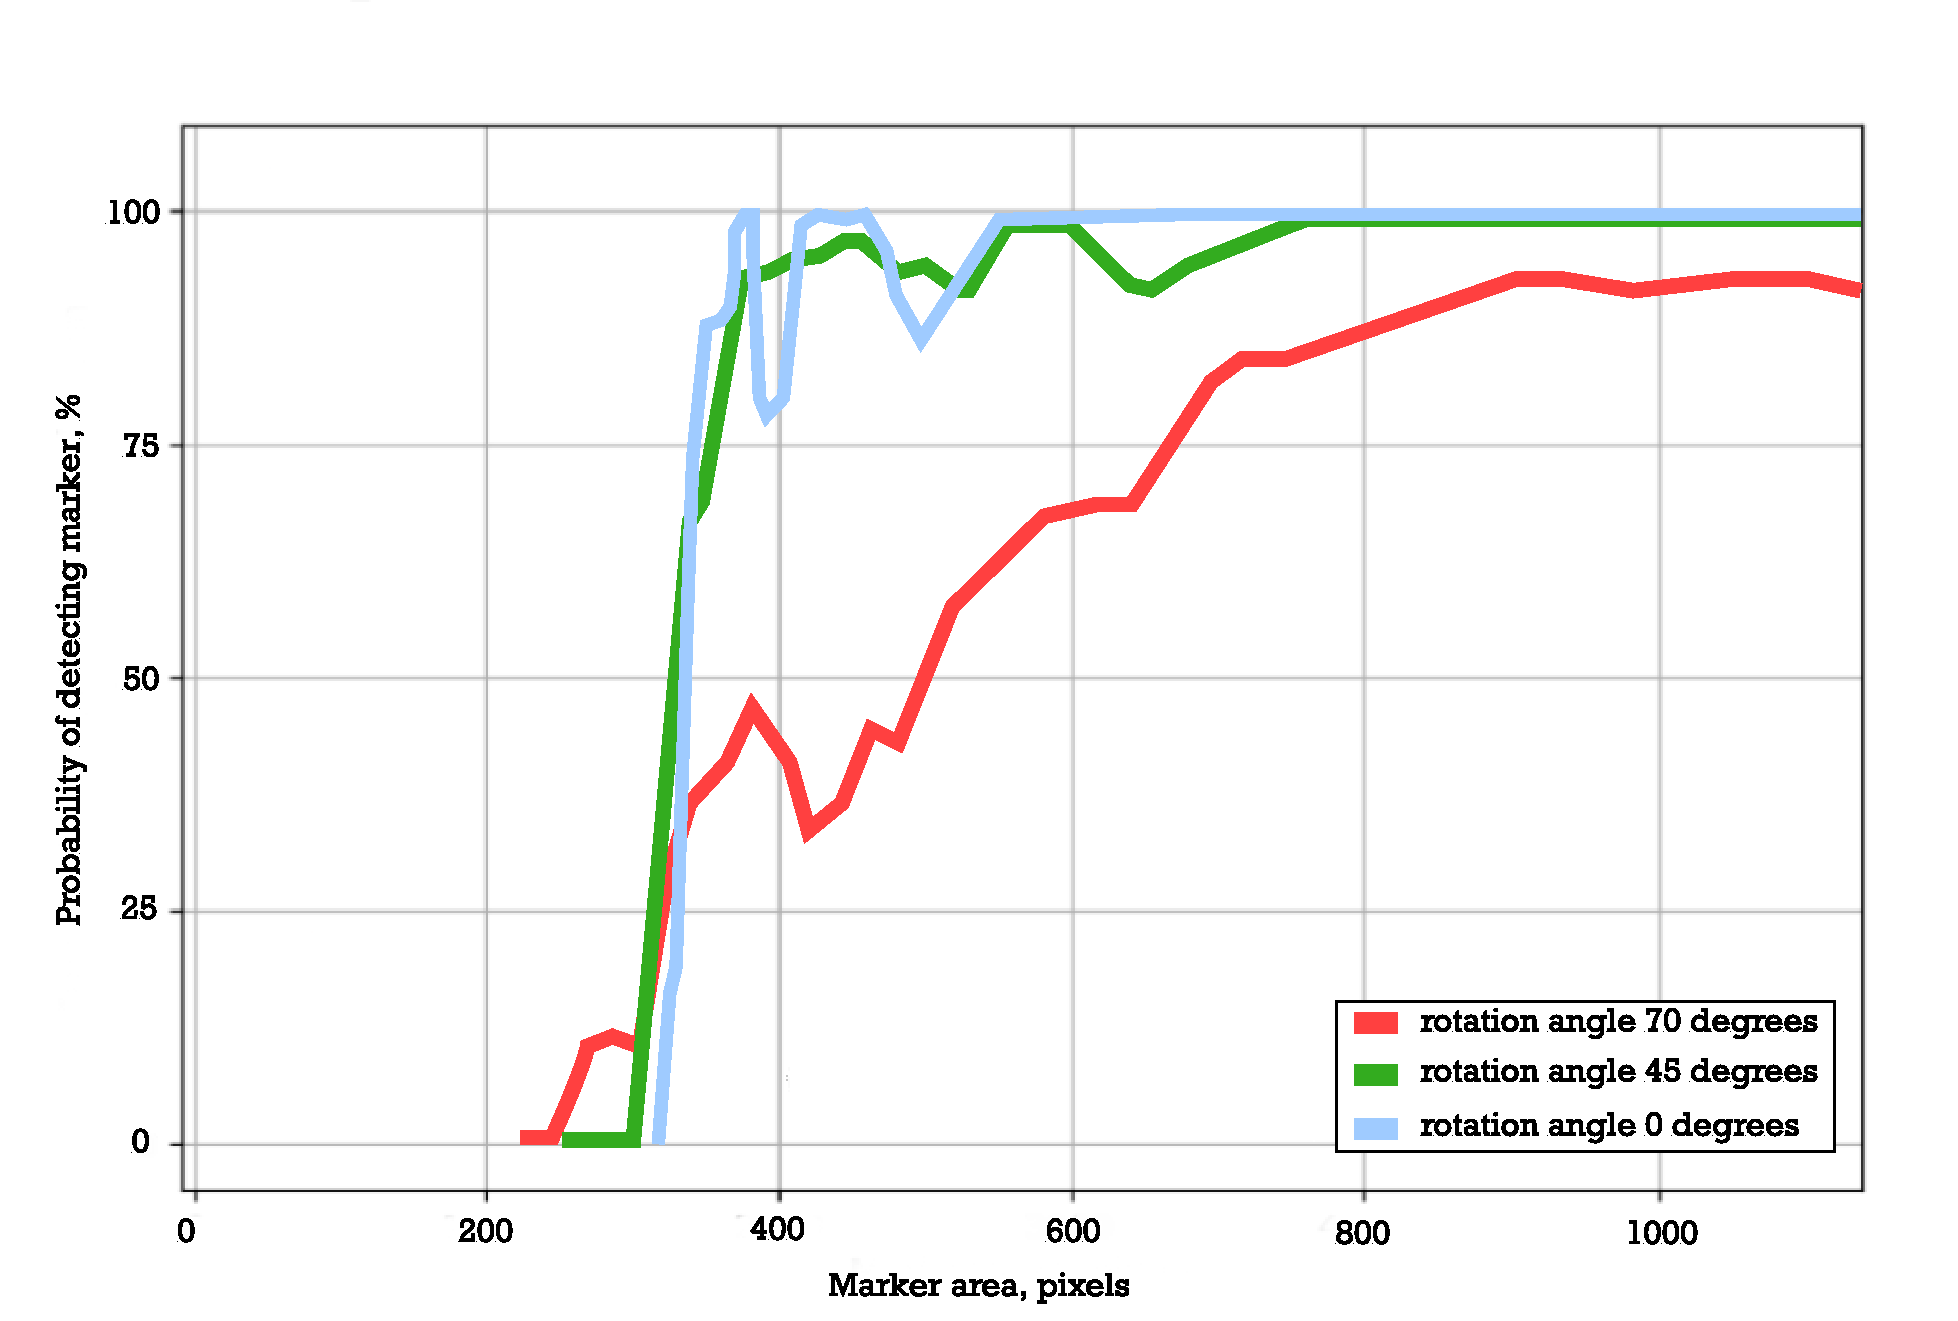
\includegraphics[width=.90\textwidth,angle=0]{figure 2-5.pdf}
    \caption{Pravdepodobnosť detekcie značky v závislosti od jej oblasti na obrázku pre 3 rôzne uhly naklonenia: 0°, 45°, 70°.}
    \captionsetup{font=footnotesize, justification=centering, skip=5pt}
    \caption*{(Zdroj: vlastné spracovanie)}
    \label{o:2-5}
\end{figure}

\begin{figure}[ht!]
    \centering
    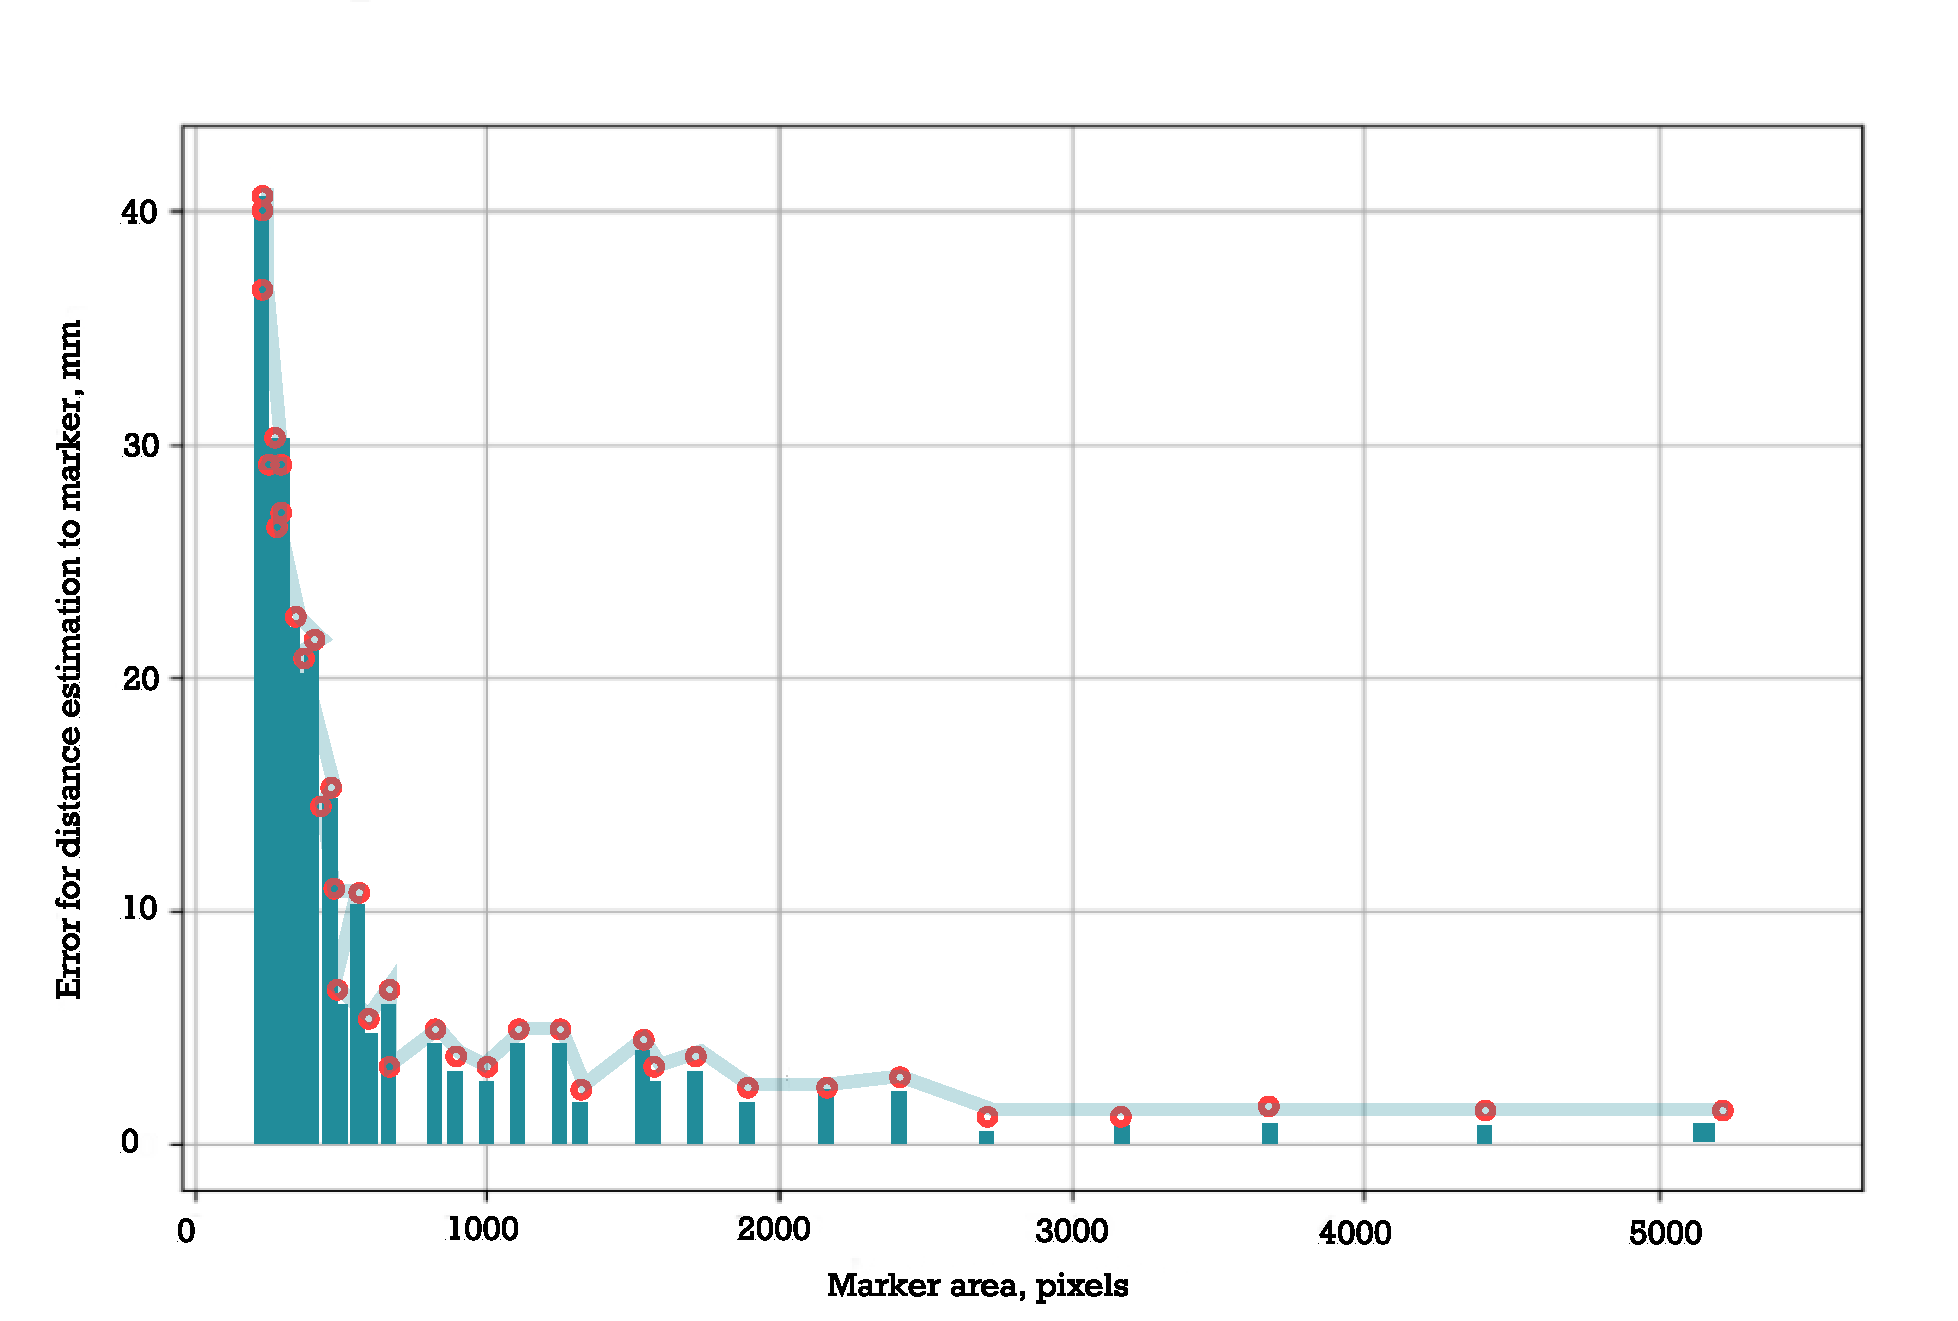
\includegraphics[width=.90\textwidth,angle=0]{figure 2-6.pdf} 
    \caption{Závislosť vplyvu veľkosti oblasti značky na chybe pri zisťovaní jej polohy.}
    \captionsetup{font=footnotesize, justification=centering, skip=5pt}
    \caption*{(Zdroj: vlastné spracovanie)}
    \label{o:2-6}
\end{figure}

V mojej súčasnej diplomovej práci budeme používať rovnakú metódu na odhad polohy dronu vybaveného jednou kamerou. Keďže metóda sa spolieha na detekciu značiek na snímkach z kamery, je dôležité zabezpečiť, aby boli značky na snímkach ľahko rozlíšiteľné a viditeľné. Ukázalo sa, že značky Aruco dobre fungujú v rôznych prostrediach a za rôznych svetelných podmienok, a preto sú vhodnou voľbou pre našu prácu \citep{Cheng2017}.

V porovnaní s predchádzajúcimi metódami, o ktorých sme hovorili, je výhodou metódy určovania polohy pomocou značiek vysoká presnosť a spoľahlivosť. Jednou z potenciálnych nevýhod používania značiek je však to, že sa musia do prostredia umiestniť vopred, čo nemusí byť praktické vo všetkých situáciách. Okrem toho sa samotné markery môžu zakryť alebo premiestniť, čo by mohlo spôsobiť problémy s dronom Napriek týmto obmedzeniam som sa rozhodol použiť túto metódu vo svojej práci kvôli jej overenej presnosti a robustnosti.

\subsection{WebSocket}
WebSocket je protokol, ktorý poskytuje plne duplexný komunikačný kanál prostredníctvom jedného spojenia TCP. Umožňuje komunikáciu v reálnom čase medzi klientom a serverom, vďaka čomu je vhodný pre aplikácie, ktoré vyžadujú časté aktualizácie alebo nízku latenciu, ako sú hry v reálnom čase, chatové aplikácie a živé dátové kanály.

V kontexte tohto projektu poskytuje použitie technológie WebSocket spôsob komunikácie dronu so serverom v reálnom čase. To je obzvlášť dôležité pre aplikácie, ktoré vyžadujú, aby dron rýchlo reagoval na príkazy alebo napríklad streamovanie videa v reálnom čase.

Jednou z hlavných výhod používania technológie WebSocket je jej nízka latencia. Na rozdiel od tradičných požiadaviek HTTP, ktoré si vyžadujú samostatnú požiadavku a odpoveď pre každú informáciu vymieňanú medzi klientom a serverom, spojenia WebSocket zostávajú otvorené a umožňujú nepretržitú komunikáciu medzi nimi. To umožňuje rýchlejšiu a efektívnejšiu komunikáciu, ktorá je ideálna pre aplikácie v reálnom čase \citep{Guan2019}.

Existuje niekoľko alternatívnych technológií, ktoré možno použiť na komunikáciu v reálnom čase, napríklad dlhé dotazovanie, udalosti odosielané serverom (SSE) a WebRTC. Dlhé dotazovanie zahŕňa nepretržité dotazovanie servera na aktualizácie, zatiaľ čo SSE umožňuje serveru posielať aktualizácie klientovi. WebRTC je komunikačný protokol typu peer-to-peer, ktorý umožňuje prenos zvuku a videa v reálnom čase \citep{Guan2019}.

WebSocket je však často uprednostňovanou voľbou na komunikáciu v reálnom čase vďaka nízkej latencii a jednoduchému používaniu. Okrem toho je WebSocket široko podporovaný modernými webovými prehliadačmi a možno ho ľahko integrovať do webových aplikácií pomocou populárnych rámcov, ako sú Node.js alebo Django.






